\documentclass{article}
\usepackage[utf8]{inputenc}
\usepackage{graphicx}
\usepackage{amsmath}
\usepackage{indentfirst}
\usepackage[a4paper, total={7in, 10in}]{geometry}
\graphicspath{ {./../res/} }
\numberwithin{equation}{section}

\title{Nanoparticles size estimation through Mie resonances}
\author{Neven Gentil}
\date{April 2022}

\begin{document}

\maketitle

\twocolumn

\section{Theory}

\subsection{Vector spherical harmonics}

First of all, let's describe the general composition of our problem: given an arbitrary particle droped in a certain medium, we hit it with a monochromatic light. With a fixed size and other specifics parameters for electromagnetic materials like the permeability $\mu$ or the complex refractive index $N$, our objective is to, theoretically, compute the electromagnetic field for the medium surrounding the particle and inside this particle itself, in order to find the expression of the scattered light.

Let's start with an arbitrary electromagnetic field represented by the couple of \textit{monochromatic} vector field $(\textbf{E}, \textbf{H})$ which satisfies the Maxwell equations:
\begin{align}
\nabla \cdot \textbf{E} &= 0\\
\nabla \cdot \textbf{H} &= 0\\
\nabla \times \textbf{E} &= i\omega \mu \textbf{H} \label{eq:rot_e} \\
\nabla \times \textbf{H} &= -i\omega \epsilon \textbf{E} \label{eq:rot_h}
\end{align}
Given the relation $k^{2} = \omega ^{2}\epsilon \mu$ and the following formula:
\begin{align}\label{eq:rot_rot_a}
\nabla \times (\nabla \times \textbf{A}) = \nabla (\nabla \cdot \textbf{A}) - \nabla \cdot (\nabla \textbf{A})
\end{align}
we obtain a couple of \textit{vector wave equation}:
\begin{align}
\nabla ^{2} \textbf{E} + k^{2}\textbf{E}&=0\\
\nabla ^{2} \textbf{H} + k^{2}\textbf{H}&=0
\end{align}
where $\nabla ^{2}$ is the vector Laplace operator, that is to say, we explicitly have $\Delta \textbf{A} = \nabla ^{2} \textbf{A} = (\nabla \cdot \nabla) \textbf{A}$.

An important thing to notice is that any vector field with zero divergence and satisfying the vector wave equation is a valid electric/magnetic field where we can obtain the corresponding magnetic/electric field by the curl (\ref{eq:rot_e})/(\ref{eq:rot_h}).

In this way, it is possible to create a vector function $\textbf{M}$ depending on a scalar function $\psi$ and an arbitrary constant vector $\textbf{c}$:
\begin{align}
\textbf{M} = \nabla \times (\textbf{c}\psi)
\end{align}
where \textbf{M} directly satisfies the condition $\nabla \cdot \textbf{M} = 0$. If we replace the expression of \textbf{M} in the vector wave equation, and thanks to (\ref{eq:rot_rot_a}), we easily obtain:
\begin{align}
\nabla ^{2} \textbf{M} + k^{2}\textbf{M} = \nabla \times [\textbf{c}(\nabla ^{2} \psi + k^{2}\psi)]
\end{align}
To satisfy the vector wave equation, $\psi$ should also satisfy the equivalent scalar wave equation:
\begin{align}\label{eq:psi_wave_eq}
\nabla ^{2} \psi + k^{2}\psi = 0
\end{align}
where, this time, $\nabla ^{2}$ is the scalar Laplace operator. By the way, as described above, if we denote $\nabla \times \textbf{N} = k \textbf{M}$, we have the perpendicular vector field of the associated artificial one, also satisfying the vector wave equation. Finally, we created the vector harmonics $\textbf{M}$ and $\textbf{N}$ with the scalar generating function $\psi$ associated to our initial electromagnetic field.

\subsection{Associated factors}

The main idea to compute all solutions required is the following: given an incident electromagnetic field, we use the boundary conditions on the surface of our particle to get all fields resulting from interaction. Thereby, it could be interesting to use the spherical polar coordinates during the calculation and particularly to express the boundary conditions. That is why we have constructed the vector harmonics above. Indeed, if we replace the constant vector $\textbf{c}$ by the radial coordinate $\textbf{r}$, $\textbf{M}$ is always a solution of the vector wave equation but, this time, for the spherical polar coordinates linked to the particle. In this way, from (\ref{eq:psi_wave_eq}), we obtain:
\begin{equation}\label{eq:wave_sph}
\begin{aligned}
\frac{1}{r^{2}}\frac{\partial }{\partial r}(r^{2}\frac{\partial \psi}{\partial r}) \quad + \\ 
\frac{1}{r^{2}sin(\theta)}\frac{\partial }{\partial \theta}(sin(\theta)\frac{\partial \psi}{\partial \theta}) \quad + \\
\frac{1}{r^{2}sin(\theta)}\frac{\partial^{2} \psi}{\partial^{2} \phi} \quad + \\
k^{2}\psi \quad = 0
\end{aligned}
\end{equation}
Obviously, from the previous formula, we can separate each variable to create $\psi$:
\begin{align}\label{eq:psi_r_t_p}
\psi(r, \theta, \phi) = R(r)\Theta(\theta)\Phi(\phi)
\end{align}
Thereby, when substitued (\ref{eq:psi_r_t_p}) into (\ref{eq:wave_sph}), we obtain three different equations, depending respectively on $r$, $\theta$ and $\phi$ which might be solved separately.

Finally, this kind of generating function $\psi$ satisfying the scalar wave equation (\ref{eq:psi_wave_eq}) is expressed in two \textit{even} ($\psi_{e}$) and \textit{odd} ($\psi_{o}$) functions as follow:
\begin{align}
\psi_{emn}&=cos(m\phi)P_{n}^{m}(cos\theta)z_{n}(kr)\\
\psi_{omn}&=sin(m\phi)P_{n}^{m}(cos\theta)z_{n}(kr)
\end{align}
where the parity of our original function is led by the $cosinus$ and $sinus$ attached with the $\phi$ variable and the \textit{angle-dependent} $m$ variable. 

The other angular part described by $\theta$ , as a \textit{Legendre's differential equation}, is solved by the \textit{associated Legendre functions} of the first kind $P_{n}^{m}(cos\theta)$ orthogonally defined on the $n$ variable. 

Moreover, the radial part, described by $r$, might be reintroduced as follow:
\begin{align}
\rho\frac{d }{d\rho}(\rho\frac{d Z}{d\rho})+[\rho^{2}-(n+\frac{1}{2})^{2}]Z=0
\end{align}
where we assume that $\rho=kr$ and $Z=R\sqrt{\rho}$. Thereby, to solve the previous equation, we can use any linear combination of the spherical Bessel functions $j_{n}$, $y_{n}$, $h^{(1)}_{n}=j_{n}+iy_{n}$ or $h^{(2)}_{n}=j_{n}-iy_{n}$: we named this kind of combination $z_{n}$.

Note that $m$ and $n$ are produced by subsidiary conditions when obtaining these three equations by rewriting (\ref{eq:wave_sph}) with separate variables: it is inherent to our physical assumptions.

In the end, we can retrieve our initial vector spherical harmonics generated by $\psi_{emn}$ or $\psi_{omn}$:
\begin{align}
\textbf{M}_{emn}=\nabla \times (\textbf{r}\psi_{emn})\\
\textbf{M}_{omn}=\nabla \times (\textbf{r}\psi_{omn})\\
\textbf{N}_{emn}=\frac{\nabla \times \textbf{M}_{emn}}{k}\\
\textbf{N}_{omn}=\frac{\nabla \times \textbf{M}_{omn}}{k}
\end{align}

At this point of the theory, it is still possible to restrain our hypothesis and more precisely the shape of the incident light. Let's consider a planar incident electromagnetic wave $E_{i}$. Now, we can easily describe this wave in terms of vector spherical harmonics:
\begin{equation}\label{eq:ei_harmo}
\begin{aligned}
\textbf{E}_{i}=\sum_{m=0}^{\infty }\sum_{n=m}^{\infty }B_{emn}\textbf{M}_{emn}+B_{omn}\textbf{M}_{omn}\\
+A_{emn}\textbf{N}_{emn}+A_{omn}\textbf{N}_{omn}
\end{aligned}
\end{equation}
where $B_{X}$ and $A_{X}$ are arbitrary factors. Thanks to the orthogonality of all the vector spherical harmonics which could be demonstrated through properties from $cos(m\phi)$, $sin(m\phi)$ and $P_{n}^{m}(cos\theta)$, we easily exctract each factor of this linear summation (\ref{eq:ei_harmo}):
\begin{align}\label{eq:bemn}
\textbf{B}_{emn}=\frac{\int_{0}^{2\pi}\int_{0}^{\pi}\textbf{E}_{i}\cdot \textbf{M}_{emn}sin\theta d\theta d\phi}{\int_{0}^{2\pi}\int_{0}^{\pi}|\textbf{M}_{emn}|^{2}sin\theta d\theta d\phi}
\end{align}
with here, for instance, the first coefficient. With the orthogonality of the sine and cosine and (\ref{eq:bemn}), we can also demonstrate that $B_{emn}$ and $A_{omn}$ vanishe for all $m$ and $n$. Then, for the same reason, $B_{omn}$ and $A_{emn}$ are nonzero only for $m=1$. Moreover, regarding their behavior and our physical assumptions, we can select the spherical Bessel function replacing $z_{n}$: we choose $j_{n}$ for its finite values close to $r=0$ and denote it as $^{(1)}$ for the associated vector spherical harmonics. Finally, we obtain:
\begin{align}
\textbf{E}_{i}=\sum_{n=1}^{\infty }B_{o1n}\textbf{M}^{(1)}_{o1n} + A_{e1n}\textbf{N}^{(1)}_{e1n}
\end{align}
Afterward, thanks to a bunch of properties from the associated Legendre functions, we deduce explicitly these two remaining factors $B_{o1n}$ and $A_{e1n}$ from (\ref{eq:bemn}) or the equivalent expression:
\begin{align}
\textbf{E}_{i}=E_{0}\sum_{n=1}^{\infty }i^{n}\frac{2n+1}{n(n+1)}(\textbf{M}^{(1)}_{o1n} - i\textbf{N}^{(1)}_{e1n})
\end{align}
Obviously, it is possible to calculate the perpendicular magnetic field $H_{i}$ with the curl (\ref{eq:rot_e}).

\subsection{Boundary conditions}

At this point, we have enough equation relative to the incident plane wave to apply the following boundary conditions:
\begin{align}\label{eq:boundaries}
(\textbf{E}_{i} + \textbf{E}_{s} - \textbf{E}_{I}) \times \overrightarrow{e_{r}} &= 0\\
(\textbf{H}_{i} + \textbf{H}_{s} - \textbf{H}_{I}) \times \overrightarrow{e_{r}} &= 0
\end{align}
where $(\textbf{E}_{s}, \textbf{H}_{s})$ and $(\textbf{E}_{I}, \textbf{H}_{I})$ are respectively the scattering and internal electromagnetic field resulting from the interaction between the incident field and our particle. Then, we assume that these last fields have the same mathematical shape, when developped in vector spherical harmonics, than $(\textbf{E}_{i}, \textbf{H}_{i})$; that is to say, the scattering and internal field are linearly dependent from the incident field up to some factors taking into account the behavior of $j_{n}$ at the boundary of our particle:
\begin{align}
\textbf{E}_{I}&=\sum_{n=1}^{\infty }E_{n}(c_{n}\textbf{M}^{(1)}_{o1n} - id_{n}\textbf{N}^{(1)}_{e1n})\\
\textbf{H}_{I}&=\frac{-k_{I}}{\omega\mu_{I}}\sum_{n=1}^{\infty }E_{n}(d_{n}\textbf{M}^{(1)}_{e1n} + ic_{n}\textbf{N}^{(1)}_{o1n})\\
\textbf{E}_{s}&=\sum_{n=1}^{\infty }E_{n}(ia_{n}\textbf{N}^{(3)}_{e1n} - b_{n}\textbf{M}^{(3)}_{o1n})\\
\textbf{H}_{s}&=\frac{k}{\omega\mu}\sum_{n=1}^{\infty }E_{n}(ib_{n}\textbf{N}^{(3)}_{o1n} + a_{n}\textbf{M}^{(3)}_{e1n})
\end{align}
Note that $^{(3)}$ means we use the spherical Bessel function of the third kind $h^{(1)}_{n}$ and $\textbf{H}_{X}$ has the same factors than $\textbf{E}_{X}$ due to the curl (\ref{eq:rot_e}). Moreover, $k_{I}$ and $\mu_{I}$ are respectively the wave vector and the permeability of the particle.

Now, we can rewrite the boundary conditions on the surface of our imaginary particle from (\ref{eq:boundaries}) with each component separated, that is to say at $r=a$ if we denote by $a$ its radius:
\begin{equation}\label{eq:boundary_comp}
\begin{aligned}
E_{i\theta} + E_{s\theta} = E_{I\theta}\\
E_{i\phi} + E_{s\phi} = E_{I\phi}\\
H_{i\theta} + H_{s\theta} = H_{I\theta}\\
H_{i\phi} + H_{s\phi} = H_{I\phi}
\end{aligned}
\end{equation}
where $E_{iX}$, for instance, denotes the $X$-component of $\textbf{E}_{i}$. Then, we apply the explicit expressions for the incident, scattering and internal field on these previous boundary conditions (\ref{eq:boundary_comp}) with, needless to say, the detailled expressions of the vector spherical harmonics $\textbf{M}_{X}$ and $\textbf{N}_{X}$. In this way, we obtain four linear equations revealing the four coefficients arbitrary pushed into $(\textbf{E}_{I}, \textbf{H}_{I})$ and $(\textbf{E}_{s}, \textbf{H}_{s})$:
\begin{equation}
\begin{aligned}
j_{n}(mx)c_{n} + h^{(1))}_{n}(x)b_{n} = j_{n}(x) \\
\mu[mxj_{n}(mx)]'c_{n} + \mu_{I}[xh_{n}(x)]'b_{n} = \mu_{I}[xj_{n}(x)]' \\
\mu mj_{n}(mx)d_{n} + \mu_{I}h^{(1))}_{n}(x)a_{n} = \mu_{I}j_{n}(x) \\
[mxj_{n}(mx)]'d_{n}+m[xh^{(1))}_{n}(x)]'a_{n} = m[xj_{n}(x)]'
\end{aligned}
\end{equation}
where the prime sign means derivation along the same argument between parenthesis. Moreover, we have the following definitions:
\begin{equation}
\begin{aligned}
x = ka = \frac{2\pi Na}{\lambda} \qquad m = \frac{N_{I}}{N}
\end{aligned}
\end{equation}
where $N_{I}$ indicates the refractive index of the particle. In the same way, $N$ is owned by the medium. By the way, it could be intersting to notice that we also have $\rho(a)=x$. 

Then, thanks to a basic Gaussian elimination, we can exctract each coefficient. Surprisingly, with some approximation on the spherical Bessel functions depending on the frequency, it is possible to admit the equality between $a_{n}$ and $d_{n}$ then $b_{n}$ and $c_{n}$. Furthermore, these two factors could be simplified by introducing the \textit{Riccati-Bessel} functions:
\begin{align}
\psi_{n}(\rho)=\rho j_{n}(\rho) \qquad \xi_{n}(\rho)=\rho h^{(1)}_{n}(\rho)
\end{align}
and we finally obtain the following expressions for the two first coefficients:
\begin{equation}\label{eq:an_bn}
\begin{aligned}
a_{n} = \frac{m\psi_{n}(mx)\psi^{'}_{n}(x)-\psi_{n}(x)\psi^{'}_{n}(mx)}{m\psi_{n}(mx)\xi^{'}_{n}(x)-\xi_{n}(x)\psi^{'}_{n}(mx)}\\
b_{n} = \frac{\psi_{n}(mx)\psi^{'}_{n}(x)-m\psi_{n}(x)\psi^{'}_{n}(mx)}{\psi_{n}(mx)\xi^{'}_{n}(x)-m\xi_{n}(x)\psi^{'}_{n}(mx)}
\end{aligned}
\end{equation}

\subsection{Cross sections}

From now on, we have enough theory to think about the experimental approach and fit all our requirements. That is to say, let's describe the coordinate system through an explicit diagram:
\begin{figure}[h]
    \centering
    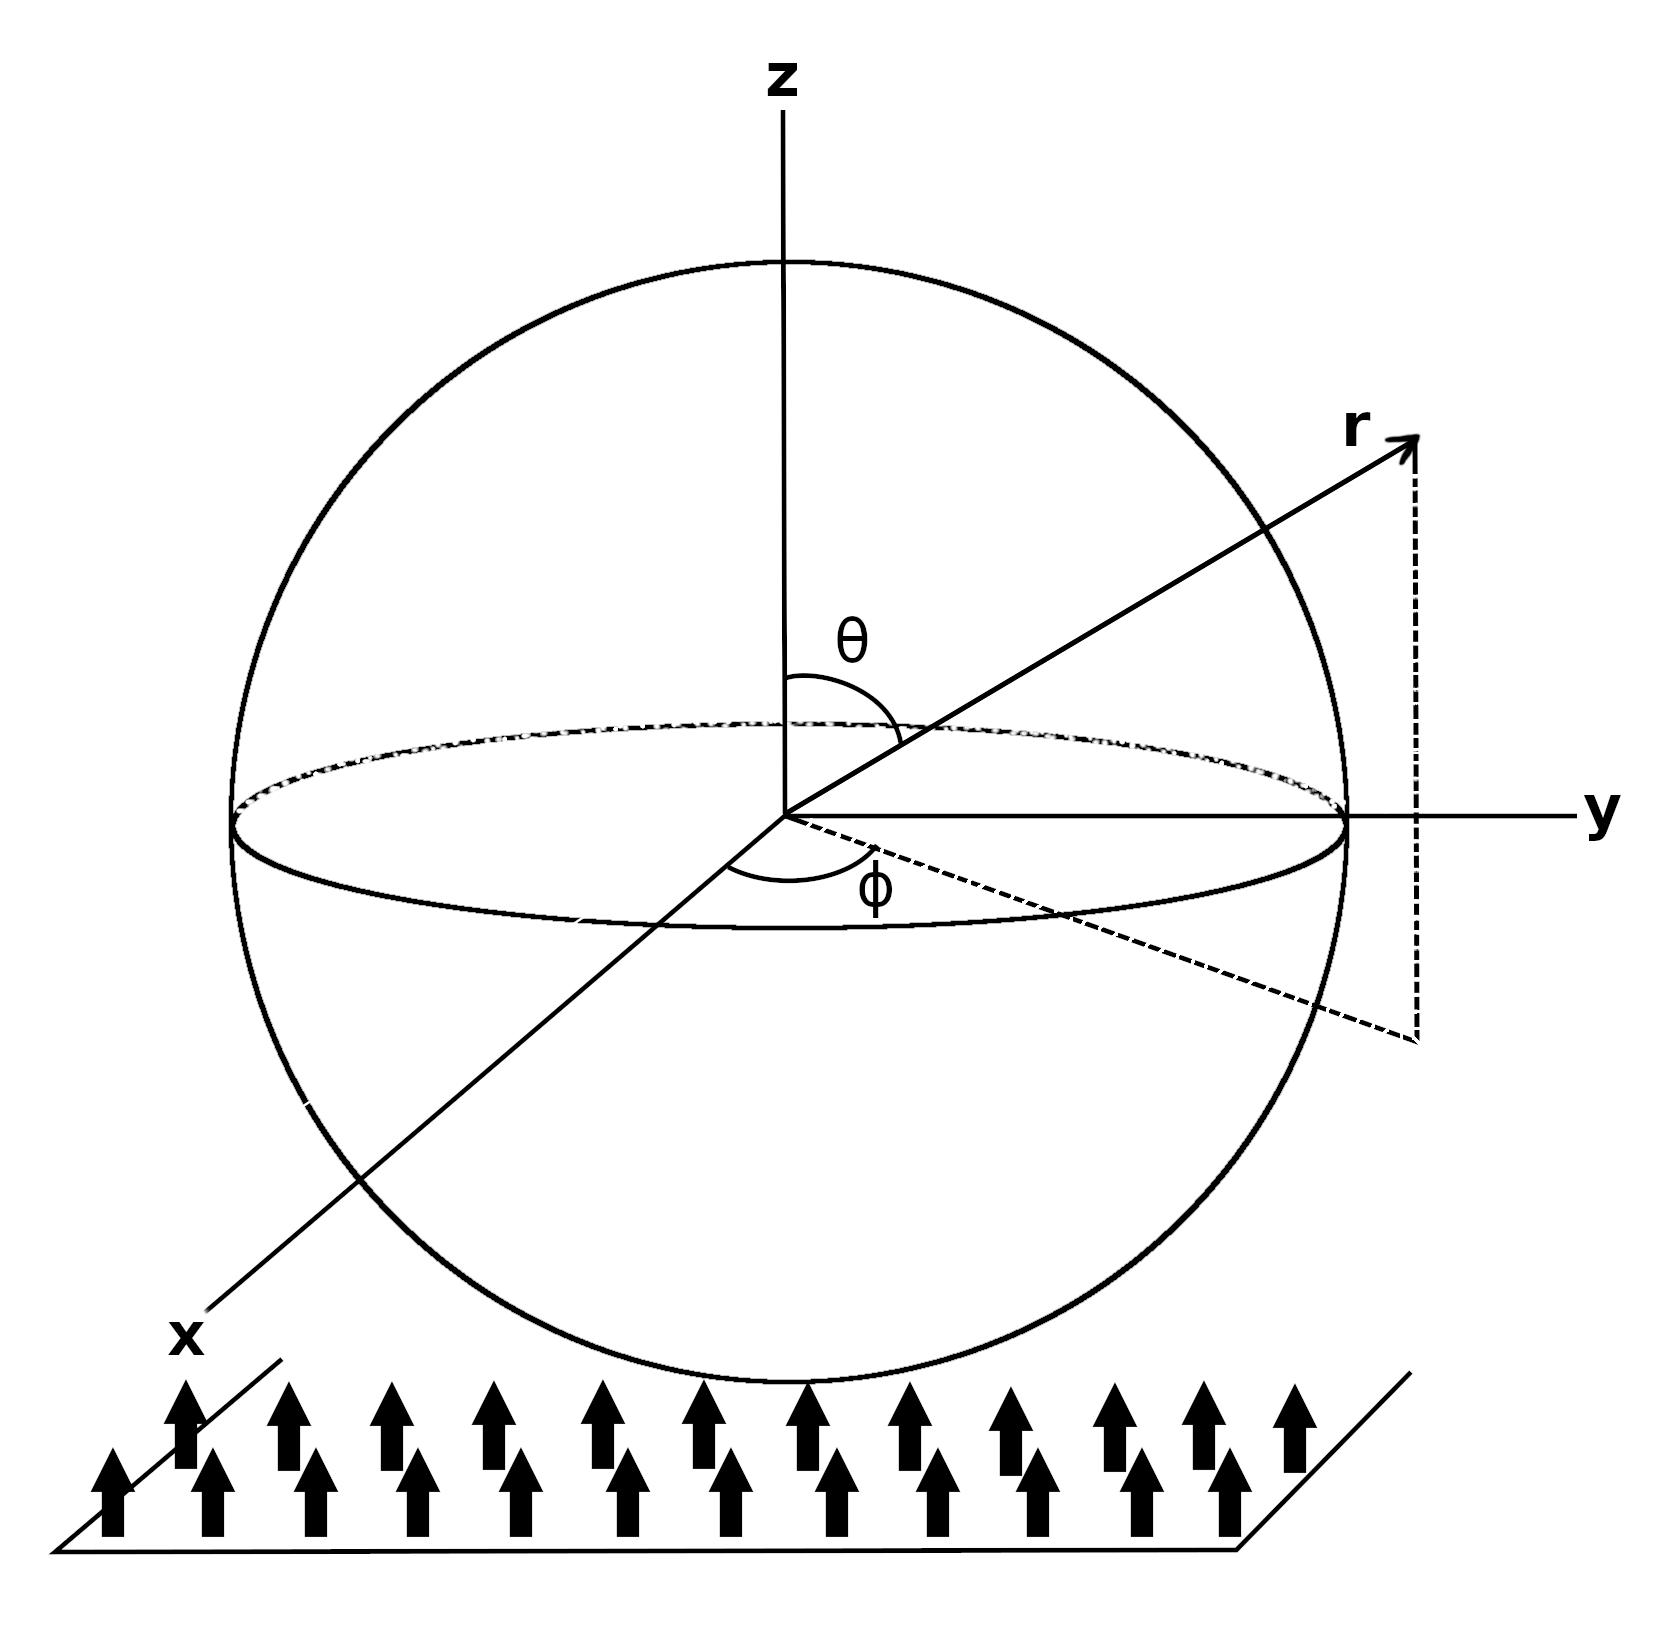
\includegraphics[width=0.4\textwidth, height=0.4\textwidth]{system.png}
    \caption{Coordinate System}
    \label{fig:system}
\end{figure}
As we can see, this reference frame is really common and our incomming plane wave is going through our particle along the z-axis. That said, our actual way to mesure the particle's size is to, roughly, retrieve the power emitted by it thanks to an optical microscope. Thereby, our goal is currently is to calculate this associated power, that is to say the net rate at which electromagnetic field crosses the surface A of an arbitrary sphere, which might be expressed as follow:
\begin{align}
W=\int_{A}^{}\textbf{S}\cdot \overrightarrow{e_{r}}dA
\end{align}
where $\textbf{S}$ is the \textit{Pointing vector} defined as:
\begin{align}
\textbf{S} = \frac{1}{2}Re\left\{\textbf{E}^{*} \times \textbf{H}\right\}
\end{align}
Note that an arbitrary sign can be added in fonction of our physical assumptions. In this way, we can now compute this power for the scattered electromagnetic field $(\textbf{E}_{s}, \textbf{B}_{s})$ and we obtain:
\begin{align}\label{eq:w_s}
W_{s}=\frac{1}{2}Re\left\{ \int_{\phi=0}^{2\pi}\int_{\theta=0}^{\pi} (E_{s\theta}H^{*}_{s\phi} - E_{s\phi}H^{*}_{s\theta})r^{2}sin\theta d\theta d\phi\right\}
\end{align}
which might be easily calculated thanks to (\ref{eq:an_bn}) included into the expression of the scattered field and, after a bit of mathematical manipulations, we have:
\begin{align}
W_{s}=\frac{\pi\left| E_{0} \right|^{2}}{k\omega\mu}\sum_{n=1}^{\infty }(2n+1)Re\left\{ g_{n} \right\}(\left| a_{n} \right|^{2}+\left| b_{n} \right|^{2})
\end{align}
where $g_{n}=(\chi^{*}_{n}\psi^{'}_{n}-\psi^{*}_{n}\chi^{'}_{n})-i(\chi^{*}_{n}\chi^{'}_{n}+\psi^{*}_{n}\psi^{'}_{n})$. This last definition can be simplified by the identity $\chi_{n}\psi^{'}_{n}-\psi_{n}\chi^{'}_{n}=1$. Moreover this power could be \textit{normalized}, that is to say, divided by the intensity from the incident light. Thereby, we introduce the associated cross section:
\begin{align}\label{eq:csca}
C_{sca}=\frac{W_{s}}{I_{i}}=\frac{2\pi}{k^{2}}\sum_{n=1}^{\infty }(2n+1)(\left| a_{n} \right|^{2}+\left| b_{n} \right|^{2})
\end{align}

In the same way, all of these previous step from (\ref{eq:w_s}) might be re-used for any other fields instead of the scattered field. Until now, only the light emitted by the particle was studied thanks to three fields: $(\textbf{E}_{i}, \textbf{H}_{i})$, $(\textbf{E}_{s}, \textbf{H}_{s})$ and $(\textbf{E}_{I}, \textbf{H}_{I})$. However, it is possible to express a variable of extinction, opposed to the scattering \textit{power} $W_{s}$, due to the interaction between the electromagnetic plane wave and our particle:
\begin{align}\label{eq:wext_ws_wa}
W_{ext} = W_{s} + W_{a}
\end{align}
This additional term, combined with the new one $W_{a}$, should be easily understood through a \textit{power balance}, that is to say an energy balance replaced by the equivalent power. Indeed, if we denote $W_{a}$ the amount of power which was varying during the interaction ($W_{a} > 0$ means that power is absorbed within the particle whereas $W_{a} > 0$ means that power is being created within the particle), it might be possible to write the following:
\begin{align}
W_{a} = W_{i} - W_{s} + W_{ext}
\end{align}
As our actual medium is nonabsorbing, $W_{i}$ vanishes identically and we retrieve the relation (\ref{eq:wext_ws_wa}). Now, the extinction \textit{power} might be evaluated in fonction of our previous vector spherical harmonic terms:
\begin{equation}
\begin{aligned}
W_{s}=\frac{1}{2}\int_{\phi=0}^{2\pi}\int_{\theta=0}^{\pi} (&Re\{E_{i\phi}H^{*}_{s\theta} - E_{i\theta}H^{*}_{s\phi}\}\; +\\
&Re\{E_{s\phi}H^{*}_{i\theta}) - E_{s\theta}H^{*}_{i\phi}\}) \\
&r^{2}sin\theta d\theta d\phi
\end{aligned}
\end{equation}
and, as stated above in (\ref{eq:csca}), we finally obtain the extinction cross section by proportionality:
\begin{align}
C_{ext}=\frac{W_{ext}}{I_{i}}=\frac{2\pi}{k^{2}}\sum_{n=1}^{\infty }(2n+1)Re\left\{a_{n} + b_{n} \right\}
\end{align}

At last, we have calculated and theoretically established the expression of two general terms which we might be retrieved by experiments: $C_{sca}$ and $C_{ext}$. It is important to note that these cross section are, not only dependent on, but also strongly linked to our hypothesis, that is to say our input variables like the refractive index. Thereby, $C_{sca}$ and $C_{ext}$ are directly reliant on the size of our studied particle.

\section{Simulations}

\subsection{Equations adjustment}

First at all, our main issue to numerically compute the cross sections $C_{sca}$ and $C_{ext}$ is to calculate the associated scattering coefficients $a_{n}$ and $b_{n}$. Globally, these two numbers are obtained through Bessel functions as we can see from (\ref{eq:an_bn}) and our goal is to retrieve each value of them between a certain range of wavlength in order to obtain a kind of spectrum. However, due to the size of our nanoparticle close to the incident wavelength included in a visible range, the variable $\rho=kr$, as a dependency for the Bessel functions, is also restrained into a small range of value close to zero along the x-axis. In fact, in the context of a computer, these targeted values could be too sensitive to be calculated with a reasonably high precision. Thereby, we could introduce the \textit{logarithmic derivative}:
\begin{align}
D_{n}(\rho)=\frac{d}{d\rho}ln[\psi_{n}(\rho)]
\end{align}
Thanks to this additional definition, we are expanding the range of hit values and decreasing the sensitivity. In this way, we can rearrange the expressions of $a_{n}$ and $b_{n}$ from (\ref{eq:an_bn}):
\begin{equation}
\begin{aligned}
a_{n}&=\frac{[D_{n}(mx)/m + n/x]\psi_{n}(x)-\psi_{n-1}(x)}{[D_{n}(mx)/m + n/x]\xi_{n}(x)-\xi_{n-1}(x)}\\
b_{n}&=\frac{[mD_{n}(mx) + n/x]\psi_{n}(x)-\psi_{n-1}(x)}{[mD_{n}(mx) + n/x]\xi_{n}(x)-\xi_{n-1}(x)}
\end{aligned}
\end{equation}
where we have used the recurrence relation:
\begin{align}
z^{'}_{n}(x)=z_{n-1}(x)-\frac{nz_{n}(x)}{x}
\end{align}
with $z_{n}$ replaced by $\psi_{n}$ or $\xi_{n}$. Note that $x$ is not a constant because of its dependency through $\lambda$ that we are going to slide along our targeted range. Moreover, due to the recurrence relations of Bessel functions explained below, in the next subsection, $D_{n}$ also satisfies the following relation:
\begin{align}\label{eq:rec_dn}
D_{n-1}(\rho)=\frac{n}{\rho}-\frac{1}{D_{n}(\rho)+n/\rho}
\end{align}
Because of the link existing between $D_{n}$ and Bessel functions, this previous recurrence (\ref{eq:rec_dn}) should be runned downwardly, that is to say begining with the higher $n$ owned by the scattering coefficients, in order to avoid the unstability of our computation as stated in the subsection below. Otherwise, the calculated data could be rapidly \textit{flawed} while $n$ is increasing.

\subsection{Computation of Bessel functions}

Useless because Python already do that. However... (recurrence relations, why unstable, solutions!)

\section{Experiments}

\section{Conclusion}

\end{document}